\documentclass[12pt]{article}
%%%%%%%%%%%%%%%%%%%%%%%%%%%%%%
%Force pdflatex processing even with "$ latex" (required by arXiv)
\pdfoutput=1
%%%%%%%%%%%%%%%%%%%%%%%%%%%%%
\usepackage[top=3cm, bottom=3cm, left=2cm, right=2cm]{geometry}
\usepackage[usenames,dvipsnames,svgnames]{xcolor}
\definecolor{darkblue}{rgb}{0.0,0.1,0.3} % dark blue
\definecolor{darkgreen}{rgb}{0,0.65,0}
\definecolor{dblue4}{rgb}{0.06,0.31,0.55} % DodgerBlue4
\definecolor{nicered}{rgb}{0.7,0.1,0.1}
\definecolor{nicegreen}{rgb}{0.1,0.5,0.1}

\usepackage[numbers,sort&compress]{natbib}
%\usepackage{cite}

\usepackage[utf8]{inputenc}
\usepackage{textcomp}
\usepackage{amsmath,amssymb,amsfonts,amsthm}
%\usepackage{siunitx} 
\usepackage{tabularx}
\usepackage{multirow}
\usepackage{dsfont}
\newcolumntype{Y}{>{\centering\arraybackslash}X}

\usepackage{xcolor}
\usepackage[colorlinks=true,citecolor= nicegreen,linkcolor=nicered]{hyperref}

\usepackage{verbatim} 
\usepackage{graphicx}
\graphicspath{{figures/}}
\usepackage{cancel}

\usepackage[colorinlistoftodos]{todonotes}

\usepackage{comment}
\includecomment{details}
\specialcomment{details}
{\begingroup}{\endgroup}
\excludecomment{details}
%\PreviewEnvironment{details}
%%%%%%
%Custom definitions
\usepackage{tikz}
\newcommand{\ReportNumbers}[1]{%
\begin{tikzpicture}[overlay, remember picture]
\path (current page.north east) ++(-1,-1) node[below left] {#1};
\end{tikzpicture}
}
%%%%%%%%%%%%%%%TITLE PAGE

\title{Dirac neutrino mass generation from Majorana messenger}

\author{First Author\footnote{\href{mailto:first@author}{first@author}},
Second Author\footnote{\href{mailto:second@author}{second@author}}\\
\textit{\small  First Institute}\\
[4mm]
Third Author\footnote{\href{mailto:third@author }{third@author}}\\
\textit{\small Second Institute}
}
\date{\small Month NN, YYYY}
\begin{document}
\maketitle
\ReportNumbers{XXX-XXX}

\begin{abstract}    
We propose a model for one-loop Dirac neutrino masses with Majorana mediators which can be dark matter candidates if they are the lightest states circulating the loop. This model is restricted by  neutrino physics,  lepton flavor violation and cosmological constrains, including  
the effective number light neutrinos $N_{\text{eff}}$. Here we find that $M_{Z^{\prime}}/g^{\prime} \gtrsim 60\ \text{TeV}$ in order to satisfy the conditions of $N_{\text{eff}}$..
\end{abstract}

\section{Introduction}
\label{sec:intro}
%Dirac or Majorana
The interpretation of neutrino experimental data in terms of neutrino
oscillations is compatible with both Majorana or Dirac neutrino masses
\cite{Tanabashi:2018oca}. The former possibility has received the most
attention but, given the lack of signals in neutrinoless double beta
decay experiments
\cite{KamLAND-Zen:2016pfg,Agostini:2018tnm,Aalseth:2017btx,Alduino:2017ehq,Albert:2017owj,Arnold:2016bed},
the latter cannot be dismissed.
% Dirac case
If neutrinos are Dirac particles, the Standard Model (SM) particle
content must be extended with right-handed neutrinos,
% with cosmology implications
which can increase the effective number of light neutrinos,
$N_{\text{eff}}$, until 6. Therefore, to be compatible with the
current cosmological restrictions on $N_{\text{eff}}$, the
interactions of the extra right-handed neutrinos with the primordial
plasma must be highly suppressed.

%Smallness of neutrinos for both Dirac and Majorana
On the other hand, to give small masses to at least two Majorana or
Dirac neutrinos, as required to explain the neutrino oscillation
experiments~\cite{Ahmad:2002jz, Fukuda:1998mi},
%focus in seesaw type I
the seesaw mechanism with heavy fermions is usually invoked.
%tree-level case
For the tree-level type-I seesaw we can have either light Majorana
neutrinos with heavy Majorana
mediators~\cite{Minkowski:1977sc,Yanagida:1979as,GellMann:1980vs,Mohapatra:1979ia}
or light Dirac neutrinos with heavy Dirac
mediators~\cite{Roncadelli:1983ty,Roy:1983be,Gu:2007mc,Ma:2014qra}.
%one-loop case
The radiative type-I seesaw includes both~\cite{Ma:2006km}
possibilities~\cite{Farzan:2012sa},
%new possibility in radiative case
but now it is also possible to have light Majorana neutrinos with
heavy Dirac mediators~\cite{Ma:2013yga}.
%New in this work
In this work we want to explore the possibility to build a simple
Dirac radiative type-I seesaw model with heavy Majorana mediators.
%Old idea but first realized here
It is worth noticing that this idea have been already illustrated in
an extension of the minimal supersymmetric standard
model~\cite{Demir:2007dt} but without show any explicit solution.

%Features of the new propossed solution
In general, solutions for light Dirac neutrino masses require a
continuous symmetry to guarantee their Diracness. This symmetry is
usually identified as the local $\operatorname{U}(1)_{B-L}$.
Additionally, ad-hoc discrete symmetries are invoked to forbid tree
level Dirac or Majorana mass terms for the light right-handed
neutrinos~\cite{Roncadelli:1983ty,Han:2018zcn,Wang:2017mcy}.
%tree-level without adhoc symmetries
However, tree-level Dirac type-I seesaw with proper choices for the
$\operatorname{U}(1)_{B-L}$ charges have been shown to be consistent
without require any extra ad-hoc discrete symmetries~\cite{Ma:2014qra}.
%one-loop 
In recent works, it has been shown that even for one-loop Dirac
neutrino masses, it is possible to have $\operatorname{U}(1)_{B-L}$ as
the only extra symmetry beyond the SM~\cite{Calle:2018ovc,Bonilla:2018ynb,Saad:2019bqf}\footnote{
%extra-loops
  For extensions with only extra scalars, minimal solutions have been found with two and three loops~\cite{Saad:2019bqf}}.
%conexion with dark matter
As a bonus in this case, the new scalars and fermions circulating the
loop can be dark matter candidates with the stability of the lightest
of them guaranteed by the very same continuous symmetry.
% remark
We focus here in solutions for the radiative Dirac type-I seesaw with
Majorana mediators, which have only an extra local symmetry responsible for the
Diracness of the light neutrinos, the absence of any tree-level
mass, and the existence of a dark sector constituted by the
particles circulating the loop.

%conexion with DM
In fact, another evidence that the SM is not a complete theory is the
missing matter content of the universe, which is known as dark matter
(DM).
% DM as particle
The main proposals that explain DM as a particle are given in
Ref.~\cite{Bertone:2004pz}.
%not found
However, there have been only gravitational evidence for the existence
of dark matter so far.
% too many possibilities
Without evidence of DM as a particle, there is not a clear path to pin
out the DM properties nor the possible heavier companions of some
extended dark sector. 
% connect with other phenomena
Linking the dark sector to other specific phenomenology allows to
reduce the arbitrariness in the model building.
% loop
In our construction, the dark sector is related to the heavy sector
responsible of the lightness of the neutrinos and the same symmetry
which guarantees the lightness of the Dirac neutrinos is the
responsible of the stability of the lightest dark particle (LDP).
% new particle prediction
Therefore, the number of specific models is quite restricted.

% We will make use of the scotogenic model~\cite{Ma:2006km}. In
% scotogenic model the neutrino masses and the DM have common
% explanation. The neutrino masses are generated by one-loop effects,
% where the candidates for DM are mediators in the loop.
%Conclusion:
In this work we propose a radiative Dirac type-I seesaw, with Majorana
fermions as mediators in the loop. This full set of mediators in the
loop can include a DM candidate.

The rest of the paper is organized as follows. In the next section we present the model and the particle content. In the section~\ref{sec:Model} we present the model and study the scalar mass spectrum after spontaneous symmetry breaking. In section~\ref{sec:Neutrinos} We present a mechanism to generate Dirac neutrino masses. In section~\ref{sec:LFV} we show the lepton flavor violation (LFV) experimental  constraints. In section~\ref{sec:DM} we present the viable DM candidates. Finally, In section~\ref{sec:CosmoConstraints} we show the cosmological restrictions ($N_{eff}$) in a nonminimum model for different extra abelian symmetries.

\section{The model}
\label{sec:Model}
%
\begin{table}[t!]
  \centering
  \begin{tabular}{|c|c|c|c|}
    \hline  
    Fields     & $\operatorname{SU}(2)_L$ & $\operatorname{U}(1)_Y $ & $\operatorname{U}(1)_X$ \\ \hline
    % $H $  & 2  1/2  &  0 \\
    $\eta$  & $\boldsymbol{2}$ & $1/2$  & $1$ \\
    $S$ & $\boldsymbol{1}$ & $0$  & $2$ \\
    $\sigma$ & $\boldsymbol{1}$ & $0$ & $3$ \\
    \hline
    % $Q_{L_{i}}$  & $(2,-1/6)$ & $0$ \\
    % $\overline{u_{R_{i}}}$ & $(1,-2/3)$ & $0$ \\
    % $\overline{d_{R_{i}}}$ & $(1,1/3)$ & $0$ \\
    % \hline
    % $L_i$  & $(2,-1/2)$ & $0$ \\
    % $\overline{e_{R_i}}$ & $(1,1)$ & $0$ \\
    $\nu_{Ri}$ & $\boldsymbol{1}$ & $0$ & $-4$\\
    $\nu_{R3}$ & $\boldsymbol{1}$ & $0$ & $5$\\
    $\psi_{R\alpha}$  & $\boldsymbol{1}$ & 0 & $1$ \\\hline
  \end{tabular}
  \caption{The new scalars and fermions with their respective charges. All the SM fields are neutral under the new $\operatorname{U}(1)_X$ gauge symmetry. }
    \label{tab:partcont}
\end{table}
%
We extend the standard model with a spontaneously broken Abelian gauge symmetry  which guarantees the total lepton number ($L$) conservation. Only the new particles including the light right handed neutrinos are charged under this symmetry. We choose the new particle set such that the following dimension six operator is realized at one-loop level
\begin{align}
  \label{eq:ld6}
  \mathcal{O}_{6D}=\frac{1}{\Lambda^2} \overline{L} \tilde{H} \nu_R S^2\,,
\end{align}
where $S$ is the singlet scalar field which spontaneously breaks the $\operatorname{U}(1)_X$ symmetry needed to forbid the Dirac and Majorana neutrino mass terms at tree level.

With the aim to illustrate the one-loop Dirac neutrino mass generation
we consider the particle content shown in Table \ref{tab:partcont} as
a possible realization of the effective operator $\mathcal{O}_{6D}$. Specifically, we introduce three scalar fields
$\eta, \sigma$ and $S$, where only $S$ develops a nonzero vacuum
expectation value (VEV),  a set of three singlet fermions,
$\nu_{Rj}$ ($j=1,2$) and $\nu_{R3}$, and another set of three heavy Majorana fermions, $\psi_{R\alpha}$ ($\alpha=1,2,3$).  
%The model also includes an additional $\operatorname{U}(1)_X$ gauge
%symmetry which is used to forbid the Dirac and Majorana neutrino mass
%terms at tree level.
%Additionally, we add three right neutrinos, one scalar doublet, two scalar singlets and three Majorana fermion singlet under $\operatorname{SU}(2)_L$.
The $\operatorname{U}(1)_X$ charges for the new particles are defined by the anomaly cancellation conditions and the gauge invariance in Yukawa and scalar interactions.
%In this model the neutrinos are Dirac fermions. Particle content and their respective charges are show in Tab.~\ref{tab:partcont}. 

The most general Lagrangian contains the following Yukawa and scalar interactions:
%
\begin{align}
\label{eq:LagY}
    \mathcal{L} \supset& -\,g_{X}\,Z_\mu^\prime\sum_{F}q_{F}\overline{F} \gamma^\mu F+\sum_{\phi}\left|\left( \partial_\mu +i\,g_{X}\,q_\phi\,Z'_\mu \right) \phi\right|^2\nonumber\\
    &-[ 
    h_{i\alpha} \overline{L_{i}} \tilde{\eta} \psi_{R\alpha} +  y_{j\alpha} \overline{\nu_{R_{j}}} \sigma^* \psi^c_{R\alpha} + \kappa_{\alpha\beta} \overline{\psi^{c}_{R\alpha}} \psi_{R\beta} S^* + \text{h.c.}] - \mathcal{V}(H, S, \eta, \sigma)\,.
\end{align}
%
In the first row $g_{X}$ is the gauge coupling associated to the $\operatorname{U}(1)_X$ group and $Z_\mu^\prime$ is its corresponding gauge boson, $F$ and $\phi$ denote the new chiral fermions and new scalars respectively, and $q_{F,\,\phi}$ their $X$ charges. In the second row
$L_{i}$ ($i=1,2,3$) and $H$ are the SM lepton and Higgs doublets, respectively,  $\widetilde{\eta} = i \sigma_2 \eta^*$, and $h$, $y$ and $\kappa$ are matrices in the flavor space. 
The scalar potential can be cast as
%
\begin{align*}
    \mathcal{V}(H, S, \eta, \sigma) = & V(H) + V(S) + V(\eta) + V(\sigma) \\
    &+  \lambda_{1} (H^{\dagger} H ) (S^{*} S) + \lambda_{2} (H^{\dagger} H ) (\sigma^{*} \sigma ) + \lambda_{3} (H^{\dagger} H ) (\eta^{\dagger} \eta )\\
    &+ \lambda_{4} (S^{*} S) (\sigma^{*} \sigma ) + \lambda_{5} (S^{*} S) (\eta^{\dagger} \eta ) + \lambda_{6} (\eta^{\dagger} \eta ) (\sigma^{*} \sigma ) + \lambda_{7} (\eta^{\dagger} H ) (H^{\dagger} \eta ) \\
    &+ \lambda_{8} (\eta^{\dagger} H S^{*} \sigma + \text{h.c.})\,,
\end{align*}
%
%
%\begin{align*}
%    \mathcal{V}(H, S, \eta, \sigma) = & \sum_{i} %V(\omega_i)+\sum_{i<j}|\omega_i|^2|\omega_j|^2+ \lambda_{7} (\eta^{\dagger} H ) %(H^{\dagger} \eta) +\lambda_{8} (\eta^{\dagger} H S^{*} \sigma + \text{h.c.})\,,
%\end{align*}
%
with $V(\omega) = \mu^{2}_{\omega} \omega^{\dagger} \omega + \lambda_{\omega} (\omega^{\dagger} \omega)^{2}$. 
Note that after the spontaneous symmetry breaking of $\operatorname{U}(1)_X$ the $\lambda_8$ term gives rise to the mixing between the neutral parts of $\eta$ and $\sigma$, which is mandatory to generate non-zero radiative masses. 
%Note that after the spontaneous symmetry breaking of $\operatorname{U}(1)_X$ the last term gives rise to the soft trilinear coupling
%\begin{align}
%  \mu=\lambda_8 \langle S \rangle\,,
%\end{align}
We assume $\lambda_8$ and $\langle S\rangle$ reals to preserve CP symmetry in the scalar sector, and $\mu^2_\eta,\mu^2_\sigma>0$ to avoid tree-level mixing terms among the fermions. 
Moreover, we also assume $\lambda_1\ll1$  such that the scalar $S$ and $H$ do not mix allowing us to identify the CP even scalar particle in $H$ as the SM Higgs boson. 
% \subsection{Scalar mass spectrum}
%\label{sec:ScaMassSpect}
To establish the scalar spectrum we expand the scalar fields as
%
\begin{align*}
  H = \begin{pmatrix}G^+ \\ \frac{1}{\sqrt{2}} (h+v_H+iG) \end{pmatrix} \,,&\hspace{1cm}
  \eta = \begin{pmatrix}\eta^{+} \\ \frac{1}{\sqrt{2}}(\eta_R+i\eta_I) \end{pmatrix} \,,\\
  S = \frac{1}{\sqrt{2}} (S_R+v_{S}+iS_I)\,,&\hspace{1cm}\sigma = \frac{1}{\sqrt{2}} (\sigma_R+i\sigma_I),
\end{align*}
%
with $v_H= 246.22$ GeV.  
%By minimizing the scalar potential we find that the mass-squared parameters $\mu_H^2$ and $\mu_S^2$
%
%\begin{align*}
%    \mu^{2}_{H} =& -\frac{1}{2}\left( \lambda_{H}  v^2 + \lambda_{1}  v_S\right)\,,  &
%    \mu^{2}_{S} =& -\frac{1}{2}\left( \lambda_{S}  v^{2}_{S} + \lambda_{1}  v^2\right)\,.
%\end{align*}
%
Of the original twelve scalar degrees of freedom in the model, the gauge bosons $W^{\pm}$, $Z^{0}$ and $Z^{\prime}$ absorb four of them (the Goldstone bosons $G^{\pm}$,$G$ and $S_{I}$). Thus, the scalar spectrum contains two sets of two neutral CP-even states ($h$ and $S_{R}$,  and $\sigma_{R}$ and $\eta_{R}$), two CP-odd scalar states ($\sigma_{I}$ and $\eta_{I}$) and one charged scalar ($\eta^{\pm}$). 
%We assume that $\lambda_{1} \ll 1$, such that the scalar $S$ and $H$ do not mix. 
The mass spectrum for the unmixed scalars reads
\begin{align*}
   & m_{\eta^{\pm}}^{2}= \mu_{\eta}^{2} + \frac{1}{2} (\lambda_{3} \upsilon^{2}_{H} + \lambda_{5} \upsilon^{2}_{S} )\,,\,\,\,\, m_{H}^{2} = \lambda_{H} \upsilon_{H}^{2}\,,\,\,\,\,    m_{S}^{2}= \lambda_{S} \upsilon_{S}^{2}\,.
\end{align*}
%
The other mass eigenstates are defined as
%
\begin{align*}
    \begin{pmatrix}\chi_{(R,I)_{1}} \\ \chi_{(R,I)_{2}} \end{pmatrix} =& \begin{pmatrix} \cos\theta & -\sin\theta \\ \sin\theta & \cos\theta \end{pmatrix} \begin{pmatrix}\sigma_{(R,I)} \\ \eta_{(R,I)} \end{pmatrix} \,,
\end{align*}
%
where $\tan\theta= 2c/(b-a)$, with $a = m^{2}_{\eta^{\pm}} + \frac{1}{2}\lambda_{7} \upsilon^{2}_{H}$, $b = \mu^{2}_{\sigma}+\frac{1}{2}(\lambda_{2} \upsilon^{2}_{H} + \lambda_{4} \upsilon^{2}_{S})$ and $c = \frac{1}{2}\lambda_8 v_{H} v_{S}$\,. Note that the CP-even  states $\chi_{R(1,2)}$ are mass degenerate with CP-odd ones $\chi_{I(1,2)}$, with masses $ m_{\chi_{(1,2)}}^{2}= [a + b \mp \sqrt{(a-b)^{2} + 4c^{2}}]/2$.   

%The other neutral mass eigenstates are defined as
%
%\begin{align*}
%    \begin{pmatrix}\chi_{(R,I)_{1}} \\ \chi_{(R,I)_{2}} \end{pmatrix} =& \begin{pmatrix} %c_{\theta_{(R,I)}} & -s_{\theta_{(R,I)}} \\ s_{\theta_{(R,I)}} & c_{\theta_{(R,I)}} \end{pmatrix} %\begin{pmatrix}\sigma_{(R,I)} \\ \eta_{(R,I)} \end{pmatrix} \,,
%\end{align*}
%
%where $\tan2\theta_{(R,I)} = \pm2c/(b-a)$, with $a = m^{2}_{\eta^{\pm}} + \frac{1}{2}\lambda_{7} %\upsilon^{2}_{H}$, $b = \mu^{2}_{\sigma}+\frac{1}{2}(\lambda_{2} \upsilon^{2}_{H} + \lambda_{4} %\upsilon^{2}_{S})$ and $c = \frac{1}{2}\lambda_8 v_{H} v_{S}$\,. 
%The corresponding mass eigenvalues are
%\begin{align*}
%   m_{\chi_{R(1,2)}}^{2} &= \frac{1}{2} \left(a + b \mp \sqrt{(a-b)^{2} + 4c^{2}} \right)\,, \\
%     m_{\chi_{I(1,2)}}^{2} &= \frac{1}{2} \left(a + b \mp \sqrt{(a-b)^{2} - 4c^{2}} \right)\,,
%\end{align*}

On the other hand, we assume that the heavy Majorana fermions are already in the diagonal basis in such a way their masses are $M_{\psi_\alpha}=\kappa_{\alpha}v_S=\sqrt{2}\kappa_{\alpha\alpha}v_S$, with $M_{\psi_1}<M_{\psi_2}<M_{\psi_3}$.
%\begin{pmatrix}
  %\psi_1 &
  %\psi_2 &
  %\psi_3
%\end{pmatrix}^{\operatorname{T}}$$

\section{Neutrino masses and charged lepton flavor violation}
\label{sec:Neutrinos}
%
\begin{figure}
\centering
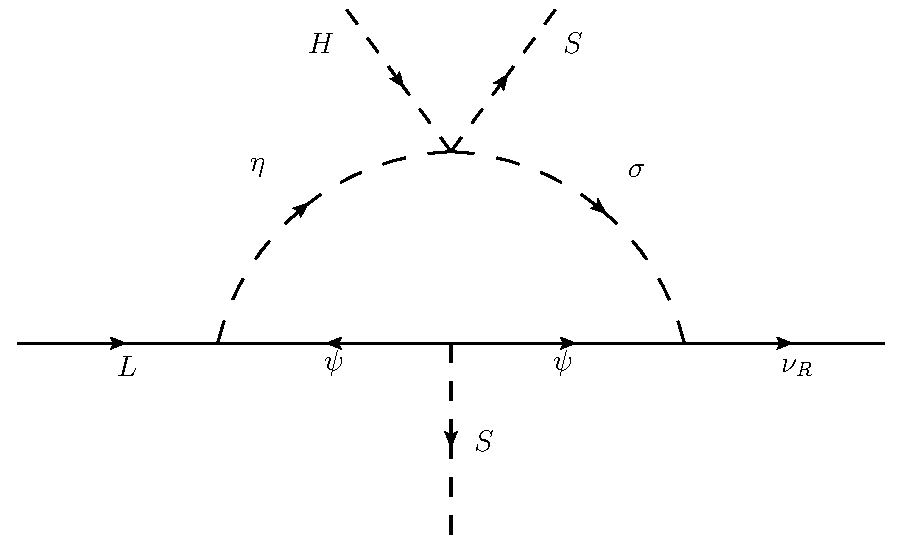
\includegraphics[scale=0.6]{Neutrino_Loop.pdf}
\caption{One-loop realization of the dimension-6 operator $\overline{L} \tilde{H} \nu_R S^2$ leading to Dirac neutrino masses with Majorana mediators.}
\label{fig:zee}
\end{figure}
%
Thanks to the scalar mixing term $\lambda_8$ nonzero Dirac neutrino masses are generated at one-loop level according to the diagram in  Fig.~\ref{fig:zee}. The expression for the effective neutrino mass matrix $\mathcal{M}_{\nu}$ can be cast as
%
\begin{align}
(\mathcal{M}_{\nu})_{ij} = \frac{1}{64 \pi^{2}}  \frac{\lambda_8 v_S^2 v_H} {m_{\chi_{R_2}}^{2}-m_{\chi_{R_1}}^{2}}\sum_{\alpha=1}^{3} h_{i \alpha} \kappa_\alpha y^{*}_{j\alpha}\left[ F\left( \frac{m_{\chi_{R_2}}^{2}}{M_{\psi_{\alpha}}^{2}} \right) - F\left( \frac{m_{\chi_{R_1}}^{2}}{M_{\psi_{\alpha}}^{2}} \right) \right] + (R \to I)\,,
%(\mathcal{M}_{\nu})_{ij} = \frac{1}{64 \pi^{2}}  \frac{\lambda_8 v_S v_H} %{m_{\chi_{R_2}}^{2}-m_{\chi_{R_1}}^{2}}\sum_{\alpha=1}^{3} h_{i \alpha} %M_{\psi_{\alpha}}y^{*}_{j\alpha}\left[ F\left( %\frac{m_{\chi_{R_2}}^{2}}{M_{\psi_{\alpha}}^{2}} \right) - F\left( %\frac{m_{\chi_{R_1}}^{2}}{M_{\psi_{\alpha}}^{2}} \right) \right] + (R \to I)\,,
\end{align}
%
%check the following formula:
where $F(x) =x \log x/(x-1)$ and $M_{\psi_\alpha}=\kappa_{\alpha}v_S$ has been used once. 
%, $M_{\psi_{a}}$ is
%the fermion mass and $\chi_{R_{(1,2)}}$ ( $\chi_{I_{(1,2)}}$ ) are the
%two CP-even (CP-odd) mass eigenstates.
%It follows that to obtain nonzero neutrino masses it is necessary that $\mu\equiv\lambda_8 %v_S \neq 0$. 
Note that the structure of the effective neutrino mass matrix, given by the
product $(M_{\nu})_{ij} \propto h_{i \alpha} y_{j\alpha}$, is similar to
the structure of the neutrino mass matrix for the tree-level seesaw
mechanism for Dirac neutrinos~\cite{Chulia:2016ngi}. 
It is also worth mentioning that if only one
fermion $\psi_R$ is added, then there will be two massless neutrinos, which
would be ruled out by the current neutrino oscillation data~\cite{deSalas:2017kay}. 
In our case, we assume the
existence of three of such fermions, generating Dirac scotogenic masses for
the two left-handed neutrinos ($\nu_{3}=\nu_{L3}+\nu_{R3}$ is massless due to the charge assignment). 

In order to estimate the possible values for the parameters involved in the neutrino masses we consider the case where $\lambda_2$, $\lambda_4$, $\lambda_7 \ll 1$ and $m_\chi^2\equiv m_{\eta^{\pm}}^2 = \mu^2_{\sigma} \gg \frac{1}{2} \lambda_8 v v_S$, which leads to $a\approx b\gg c$. 
Taking into account that for the mentioned case $m^2_{\chi_{R_{2}}}-m^2_{\chi_{R_{1}}} = \lambda_8 v v_{S}$ and $m^2_{\chi_{R_{2}}}+m^2_{\chi_{R_{1}}} = 2 m^2_\chi$, we have that
%
\begin{align*}
(\mathcal{M}_{\nu})_{ij} = \frac{\lambda_8 v_S^2 v}{32 \pi^{2}} \sum_{\alpha=1}^{3} \frac{h_{i \alpha} \kappa_\alpha y^{*}_{j\alpha}} {m_\chi^{2}-M_{\psi_{\alpha}}^{2}} \left[1 - \frac{M_{\psi_{\alpha}}^{2}}{m_\chi^{2}-M_{\psi_{\alpha}}^{2}} \log \left( \frac{m_{\chi}^{2}}{M_{\psi_{\alpha}}^{2}} \right)\right]\,,
\end{align*}
%
and by furhter assuming $m_{\chi}^{2} \gg (\kappa_\alpha v_S)^2$ one finds 
%
\begin{align}
(\mathcal{M}_{\nu})_{ij} & = \frac{\lambda_8 v_S^2 v}{32 \pi^{2}m_{\chi}^{2}} \sum_{\alpha=1}^{3} h_{i \alpha} \kappa_{\alpha}y^{*}_{j\alpha}\,, \\
& \sim 0.04~\text{eV} \left( \frac{\lambda_8}{10^{-4}}\right) \left( \frac{v_{S}}{200\,  \text{GeV}}\right)^2 \left( \frac{\kappa_\alpha}{0.5}\right) \left( \frac{2\, \text{TeV}}{m_{\chi}}\right)^{2} \left( \frac{h_{i \alpha} y_{j\alpha}}{10^{-4}}\right)\,. \nonumber
\end{align}
%
In this way, in addition to the loop suppression it is possible to 
have further suppression in the neutrino mass matrix for small values
of either $v_S$, $\lambda_8$ or $h_{i \alpha} y_{j\alpha}$.

%The mass matrix for Dirac neutrinos is diagonalized by
%\begin{align*}
%(U^{\nu}_R)^{\dagger} \mathcal{M}_{\nu} U^{\nu}_L = \mathcal{M}_{\nu}^{\text{diag}} = %\text{diag}(m_1, m_2, m_3)\,,
%\end{align*}
%where $U^{(\nu)}_R$ and $U^{(\nu)}_L$ are the unitary $3 \times 3$
%matrices associated to the right-handed and left-handed neutrino sectors. The leptonic %charged currents with non-massless neutrinos
%are parametrized in terms of the unitary mass
%\begin{align*}
%U_{\text{PMNS}} = \left( U^{\ell}_L \right)^{\dagger} U^{\nu}_L\,,
%\end{align*}
%where is the left diagonalization matrix of the charged leptons.
%As we already are in the diagonal basis after the calculation of the
%one-loop neutrino masses, we can set
%$U_{L}^{\ell} = \mathds{1}$. Moreover, we assume that $U_{R}^{\nu} = \mathds{1}$.
%Therefore, we can express the Dirac neutrino mass matrix in the
%following way
%\begin{align}
%(\mathcal{M}_{\nu})_{ij} = (U_{\text{PMNS}})_{ij} (\mathcal{M}_{\nu}^{\text{diag}})_{j}\,,
%\end{align}
%where the matrix $U_{\text{PMNS}}$ is expressed in the standard parameterization as
%\begin{align*}
%U_{\text{PMNS}} = \begin{pmatrix}
%    1 & 0		& 0 \\
%    0 & c_{23}  & s_{23} \\
%    0 & -s_{23} & c_{23}
%\end{pmatrix}
%\begin{pmatrix}
%    c_{13}  &  0 & s_{13}e^{-i\delta} \\
%    0 		&  1 & 0 \\
%    -s_{13}e^{i\delta} &  0 & c_{13}
%\end{pmatrix}
%\begin{pmatrix}
%    c_{12}  & s_{12} & 0 \\
%    -s_{12} & c_{12} & 0 \\
%    0		& 0		 & 1
%\end{pmatrix}\,,
%\end{align*}
%where $s_{ij} = \sin \theta_{ij}$ and $c_{ij} = \cos \theta_{ij}$ and $\theta_{ij}$ are %neutrino mixing angles and $\delta$ is CP-violating phase.

%\section{Lepton flavor violation}
%\label{sec:LFV}

On the other hand, the $h_{i\alpha}$ Yukawa interaction in Eq.~\eqref{eq:LagY} leads to charged lepton flavor violation (CLFV) processes induced at one-loop level and mediated by the charged scalars $\eta^{\pm}$) as the ones shown in Fig.~\ref{fig:LFV} for the $\ell_i\to\ell_j\gamma$ type. 
current experimental constraint on Br$(\mu \to e\gamma)$ \textless $5.7 \times 10^{-13} $~\cite{Adam:2013mnn} and for the case $m_\chi^2=m_{\eta^{\pm}}^{2} \gg M_{\psi_{a}}^{2}$
 we obtain an upper bound for the Yukawa couplings product (for a given $m_\chi$)
\begin{align}
    \left| \sum_{\alpha}h_{i \alpha} h_{j\alpha}^{*} \right| \lesssim 0.02 \left(\frac{m_\chi}{2\,\text{TeV}} \right)^{2}.
\end{align}
It is worth noticing that $y_{j\alpha}$ is not constrained by the non observation of LFV processes. 

%
\begin{figure}[t]
\centering
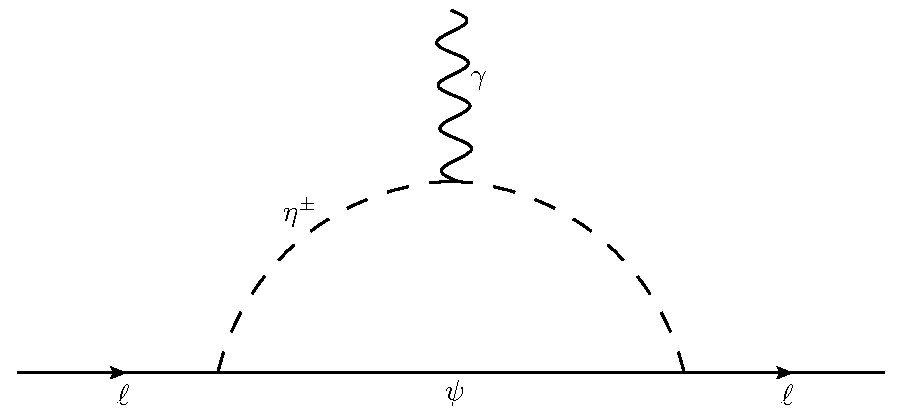
\includegraphics[scale=0.6]{LFV.pdf}
\caption{Feynman diagram for the processes $\ell_{i} \to \ell_{j} \gamma$}
\label{fig:LFV}
\end{figure}
%


%
%which leads to a very slight requirement,

%The most common search for CLFV focuses on the $l^{-}_{i} \to l^{-}_{j} \gamma$ process. This process is described by the effective Lagrangian
%
%\begin{align}
%    \mathcal{L} = \frac{\mu_{m}^{\alpha \beta}}{2} l^{-}_{\beta} \sigma^{\mu \nu} l^{-}_{\alpha} F_{\mu \nu}
%\end{align}
%
%where $\mu_{m}^{\alpha \beta}$ is a transition magnetic moment~\cite{Toma:2013zsa}.
%The decay rate is given by~\cite{Lavoura:2003xp}
%
%\begin{align}
% \Gamma(l^{-}_{i} \to l^{-}_{j} \gamma) = \frac{m^{3}_{i}}{16 \pi} \left| \sum_{\alpha} h_{i \alpha} m_{i} h_{\alpha j} \frac{i e}{16 \pi M^{2}_{\eta^{-}}} K(t_{k}) \right|^{2}\,, 
%\end{align}
%
%where $t_{\alpha} = M^{2}_{\psi_{\alpha}}/M^{2}_{\eta^{-}}$ and
%
%\begin{align}
%    K(t_{\alpha}) = \frac{2t_{\alpha}^{2}+5t_{\alpha}-1}{12(t_{\alpha}-1)^{3}} - %\frac{t_{\alpha}^{2}\log t_{\alpha}}{2(t_{\alpha}-1)^{4}}\,.
%\end{align}
%
%If we assume that $t_{\alpha} \to 0$, $t_{\alpha} \to 1$ and $t_{\alpha} \to \infty$, we have that $K(t_{\alpha}) = 1/12$, $K(t_{\alpha}) = 1/24$ and $K(t_{\alpha}) = 1/(6t)$, respectively.

%For $i \neq j$ we have CLFV processes, these processes are severely restricted by the current bounds , which set limits to the Yukawas. The most restrictive experimental bounds is decay $\mu \to e \gamma$, which is several orders of magnitude greater than radiative decays $\tau \to~l\gamma$, with $l = e, \mu$. These restrictions are given by Br$(\mu \to e\gamma)$ \textless $5.7 \times 10^{-13} $~\cite{Adam:2013mnn}, Br$(\tau \to e\gamma) $\textless$ 3.3 \times 10^{-8}$ and Br$(\tau \to~\mu\gamma) $\textless$ 4.4 \times 10^{-8}$~\cite{Aubert:2009ag, Bona:2007qt, Miyazaki:2012mx}. 

%In the limit $m_{\eta^{\pm}}^{2} \gg M_{\psi_{a}}^{2}$, $t_{\alpha} \to 0$ the decay width reads
%
%\begin{align}
% \Gamma(l^{-}_{i} \to l^{-}_{j} \gamma) = \frac{m^{3}_{i}}{16 \pi} \left| \sum_{\alpha} h_{i \alpha} m_{i} h_{\alpha j} \frac{i e}{16 \pi M^{2}_{\eta^{-}}} \left[ \frac{1}{12} \right] \right|^{2}\,, 
%\end{align}
%
%using the current experimental constraint to Br$(\mu \to e\gamma)$, can be fullfilled provided
%
%\begin{align*}
%    \left( \sum_{\alpha} \frac{h^{}_{i \alpha} h_{\alpha j}^{*}}{M^{2}_{\eta^{-}}} \right)^{2} \leq 5.7 \times 10^{-13} \frac{768 \pi G_{F}^{2}}{\alpha_{EM}}
%\end{align*}
%
%which leads to a very slight requirement,
%\begin{align*}
%    \left| \sum_{\alpha}h^{}_{i \alpha} h_{\alpha j}^{*}\left(\frac{50\text{TeV}}{M^{2}_{\eta^{-}}} \right)^{2} \right| \leq 12.65
%\end{align*}
%
%For $i = j$ we have processes that contribute to the leptonic magnetic dipole moment. In the case of the anomalous muon magnetic dipole moment, the experimental measurements does not agree with the values predicted by the SM~\cite{Lindner:2016bgg}. This can be a proof of the veracity of the model, in addition to giving restrictions on the Yukawas.

\section{Dark matter}
\label{sec:DM}
From the model charge assignment in Table~\ref{tab:partcont} we have that a residual $Z_2$ symmetry is left over after the $\operatorname{U}(1)_X$ symmetry breaking, with the particles circulating the one-loop neutrino mass diagram  (see Fig.~\ref{fig:zee}) and $\nu_{R3}$ being odd under it whereas $\nu_{R1}, \nu_{R2}$ and all the SM particles trivially transforming. Thus the lightest electrically-neutral $Z_2$-odd particle becomes a dark matter candidate. In other words, this model also provides a solution to the DM puzzle via either fermion ($\psi_1$) or scalar ($\chi_{1R}$ or $\chi_{1I}$) dark matter\footnote{Note that $Z'$ can not constitute a DM candidate due to the instability associated to the $Z'\to\bar{\nu}_{R3}\nu_{R3}$ decay channel, since it can not be kinematically closed.}. 

%\subsection{Fermion dark matter}
Since $\psi_{1}$ is a singlet under the SM gauge group its thermal relic density is controlled by the Yukawa and $\operatorname{U}(1)_X$ gauge interactions. 
The scenario where $\psi_{1}$ self-annihilates dominantly through $h_{i\alpha}$-mediated interactions resembles the very well known scotogenic model \cite{Ma:2006km},  
where sizable $h_{i\alpha}$ are required to reproduce the correct DM abundance, which in turn leads to a mild tension with experimental upper bounds on the rates for rare charged lepton decays~\cite{Kubo:2006yx,Sierra:2008wj,Ibarra:2016dlb}. 
%The phenomenology of this scenario has been extensively studied  \cite{Kubo:2006yx,Sierra:2008wj,Suematsu:2009ww,Gelmini:2009xd,Hambye:2009pw,Aoki:2010tf,Schmidt:2012yg,Ma:2012if,Kashiwase:2012xd,Kashiwase:2013uy,Racker:2013lua,Toma:2013zsa,Molinaro:2014lfa,Vicente:2014wga,Merle:2015gea,Merle:2015ica,Merle:2016scw,Hagedorn:2016dze,Lindner:2016kqk,Hessler:2016kwm,Ibarra:2016dlb}.
On the other hand, when the $Z'$ portal \cite{Langacker:2008yv,Arcadi:2013qia} is the main gate to visible sector, $\psi_1$ largely annihilates into neutrinos in such a way the observed DM abundance can be reproduced without entering in conflict with the DM searches, which follows from the fact that the $Z'$ does not couples to quarks neither to charged leptons)
(see~\cite{Arcadi:2013qia,Alves:2013tqa,Alves:2015pea,Alves:2016cqf,Blanco:2019hah} for phenomenological studies on $Z'$-mediated Majorana DM). 
% check Ibarra papers
%also through the annihilation
%$\psi_{1} \psi_{1} \to l _{\alpha}^+ \overline{l}_{\beta}^- $, via 
%Yukawa coupling $h^{a}_{i}$. These Yukawa couplings are restricted by
%CLFV and neutrino masses. %But, Yukawa couplings $y^{a}_{j}$ is free.
%In the case where the mass of the other fermions and scalars is nearly
%degenerated to $\psi_{1} $, the processes of coannihilation can be
%relevant for the relic density calculation~\cite{Klasen:2013jpa}.

%   Because the particle $\psi_{1}$ only interacts with the leptons via the Yukawa couplings, this model has no a direct detection cross section at three level. 

% In the case that the mass of the lightest fermion $\psi$ is smaller
% than the mass of the scalars, the DM will be fermionic. For this DM it
% is possible to have the following observable decay of the scalar
% $\eta^{\pm} \to l^{\pm} \psi_{1}$, therefore, the other fermions decay
% as $ \psi \to l^{\pm} l^{\mp} \psi_{1}$ and
% $\psi \to l^{\pm} l^{\mp} \psi_{1,2} $, through $\eta^{\pm}$.

%\subsection{Scalar dark matter}
In contrast to fermion DM, the scalar DM candidate has additional interaction terms to the Yukawa and gauge interactions. This entails that the later ones can be used to alter the relic density predictions in scenarios with mixed scalar DM. Since in the present model the CP-even and CP-odd neutral $Z_2$-odd particles are mass degenerate, we have the scenario of singlet-doublet complex DM~\cite{Kadastik:2009dj,Belanger:2012vp} where the DM candidate is a mixture of a complex singlet \cite{McDonald:1993ex} and a $SU(2)_L$ doublet \cite{Deshpande:1977rw,Barbieri:2006dq}. It follows that for negligible Yukawa and gauge interactions there are two DM mass regions that allow us to properly reproduce the relic abundance, one corresponds the Higgs funnel region and the second one demands masses above $100$ GeV~\cite{Kakizaki:2016dza}. 

%This corresponds to the simplified dark matter model of scalar singlet-doublet dark matter, which have been studied in detail in~\cite{Restrepo:2019soi} 

%When the lightest scalar  is mainly a scalar doublet, the phenomenology will be similar inert doublet model~\cite{Honorez:2010re}. For this kind of DM model  inert doublet model there are two mass regions for DM which can to reproduce adequately the relic density ($50$GeV \textless $m_{DM}$ \textless $70$GeV and $535$GeV \textless $m_{DM}$ \textless $20$TeV)~\cite{Garcia-Cely:2015khw}.

% In recent studies, these two regions are connected through use of a
% second doublet~\cite{Borah:2019aeq}. How we have in the model the
% Yukawa coupling, the decay $\psi_{i} \to l^{\pm} \eta^{\mp}$ is
% possible. In addition, decay is given via scalar interactions
% $\eta^{\pm} \to \eta^{0} + {W^{\pm}}$, where $W^{\pm}$ can be real or
% virtual and decay to leptons or quarks.

%Now, if the lightest scalar is mainly a singlet, the DM will be similar to Singlet %Scalar Dark Matter Model~\cite{Athron:2017kgt}\todo{change for the original ref by Ma et al. etc}.
%The mass range for the scalar singlet that produces the adequate relic
%density is around the Higgs resonance and for masses above $1$TeV. For
%this model~\cite{}, the relevant coupling for DM phenomenology is the
%Higgs portal trough the Lagrangian term $\sigma^{2} H^{2}_{i}$.
%This term generates interesting phenomenological consequences.
%Such as, thermal production of DM in the early
%universe~\cite{Yaguna:2008hd}, direct detection and invisible decay of
%SM Higgs through $h \to \sigma \sigma$~\cite{Mambrini:2011ik}.
%In addition, this model has important contributions for cosmology, in
%phenomena such as inflation~\cite{Lerner:2009xg} and
%baryogenesis~\cite{Cline:2012hg}.

\section{Beyond the minimal model: cosmological constraints}
\label{sec:CosmoConstraints}
A not-so-minimal model can be obtained by introducing additional chiral SM singlet fields. 
In this case we can use the solutions to the anomaly cancellation conditions found for an Abelian gauge symmetry $\operatorname{U(1)_X}$ in~\cite{Jenkins:1987ue,Appelquist:2002mw,Campos:2017dgc,Okada:2018tgy,Jana:2019mez}.
We use $f$ ($f$) to denote the $X$-charge of the field $f_R$ ($F_L$) for one generation of the SM. The three linear anomalies in $\operatorname{U(1)_X}$ allows to express three $X$-charges in terms of the other two
\begin{align}
  u=&-e+\frac{2l}{3}\,,& d=& e-\frac{4l}{3}\,,& q=& -\frac{l}{3}\,.
\end{align}
The quadratic anomaly condition is automatically satisfied, while the mixed gauge-gravitational and cubic anomalies depend of any extra singlet quiral fermions of zero hypercharge, like the right-handed counterpart of the Dirac neutrinos. For $\alpha$ extra quiral fields with $X$-charge $n_{\alpha}$, these conditions read
\begin{align}
  \sum_{\alpha} n_{\alpha}+3 (e-2l)=&0\,, &   \sum_{\alpha} n_{\alpha}^3+3 (e-2l)^3=&0\,. &
\end{align}
There are many known solutions for the case in which $e-2l=1$. The full set of standard model charges in terms of $l$ is just
\begin{align}
  u=&-1-\frac{4l}{3}\,,&d=&1+\frac{2l}{3}\,,&q=&-\frac{l}{3}\,,&e=&1+2l\,,&h=&-1-l\,.
  \label{Eq:SMCharges}
\end{align}
The same solution but in terms of $h$ is given in ~\cite{Okada:2018tgy}.

For this kind of solutions we have that
\begin{align}
  \psi=&-\frac{\nu+1}{4}\,,&\eta=&-\frac{\nu+1}{4}-l\,,&\sigma=&\frac{1-3\nu}{4}\,.
\end{align}



We are interested here in the case of the exotic set of $X$-charges
charges: $\mp 4$,~$\mp 4$,~$\pm 5$, that when assigned to the
three light right-handed neutrinos can forbid three level Dirac and
Majorana masses~\cite{Calle:2018ovc}. This set is compatible with the
Abelian gauge groups $X=B-L,R,D,G$ defined in~\cite{Campos:2017dgc}\footnote{We change $\operatorname{U}(1)_B$ for the more suitable name of $\operatorname{U}(1)_R$~\cite{Jana:2019mez}}.
The presence of a set of heavy Majorana mediators to realize the
dimension-5 operator at one-loop with the diagram in
fig.~\ref{fig:ld5}., would spoil the anomaly cancellation conditions.
However, we can further add an extra set of quiral fermion in a
vector-like way, such that the full set heavy fermions do not affect
the anomaly cancellation. A such assignment is displayed in
Table~\ref{tab:partcont2}.
The fields $\xi_{L \alpha}$ guarantee the anomaly cancellation and
their Majorana masses are obtained in the same way than the ones for
$\psi_{R\alpha}$.



In this way we end up with a model with four Majorana fermions, two more than in the minimal solution. Alternatively we can have a single set of $\psi_R$ and $\xi_L$ but two set of scalars $\eta_\alpha$, $\sigma_{\alpha}$~\cite{Reig:2018mdk}. If we choose $r$ as a fraction with denominator $4$, let say $r=3/4$, the $\operatorname{U}(1)_{B-L}$ left out a remnant $Z_2$ discrete symmetry which guarantees the stability of the lightest odd-particle.

The two additional left-handed fields $\xi_{L\alpha}$,  with a $\operatorname{U}(1)_{B-L}$ charge of $r=3/4$,  cancel out the anomalies. Moreover, we have both Dirac mass terms $\overline{\xi_{L \alpha}}\psi_{R \beta}$ and $ \overline{\xi_{L\alpha}^c }\xi_{L \beta} \langle S\rangle$ and the full set of Majorana fields are massive and heavy. The lighter of them a would be dark matter candidate.

%the charges for the SM particles are in equations~\ref{Eq:SMCharges}. Since these are determined by the anomaly cancellation equations.
%For this operator we have that the charges for the new particles are given by
%\begin{align}
%    \psi=&-\frac{\nu+1}{4}\,,&\eta=&-\frac{\nu+1}{4}-l\,,&\sigma=&\frac{1-3\nu}{4}\,.
%\end{align}
%As we are interested here in the case of the exotic set of X-charges charges:$\mp 4$,$\mp 4$,$\pm 5$, the charges for the model particles are shown in the table~\ref{tab:partcont3}.
%Because the charges of the SM fermions are the same for both operators ($5d$ and $6d$), the $N_{eff}$ restrictions shown in the figure~\ref{fig:Neff} apply to both operators.
%
\begin{table}
  \centering
  \begin{tabular}{|c|c|c|c|c|c|c|c|}
    \hline  
    Fields     & $\operatorname{SU}(2)_L$ &  $\operatorname{U}(1)_Y $ & $\operatorname{U}(1)_{X}$& $\operatorname{U}(1)_{B-L}$& $\operatorname{U}(1)_R$& $\operatorname{U}(1)_D$& $\operatorname{U}(1)_G$\\ \hline
$L $     & $\boldsymbol{2}$ & $-1/2$ & $l$      &  $-1$&    $0$ &  $-3/2$&  $-1/2$ \\    
$d_R $   & $\boldsymbol{1}$ & $-1/2$ & $1+2l/3$ &  $1/3$&    $1$&  $0$&  $2/3$ \\
$u_R $   & $\boldsymbol{1}$ & $+2/3$ & $-1-4l/3$&  $1/3$&   $-1$&  $1$&  $-1/3$ \\
$Q $     & $\boldsymbol{2}$ & $-1/6$ & $-l/3$   & $1/3$&    $0$&  $1/2$&  $1/6$ \\\hline
$e_R $   & $\boldsymbol{1}$ & $-1$   & $1+2l$   &  $-1$&    $1$ &  $-2$&  $0$ \\
$H $     & $\boldsymbol{2}$ & $1/2$  & $-1-l$   &  $0$&    $-1$ &  $1/2$&  $-1/2$ \\
$\eta$   & $\boldsymbol{2}$ & $+1/2$ & $3/4-l$  & $7/4$& $3/4$ &$9/4$&$5/4$ \\
$S$      & $\boldsymbol{1}$ & $0$    & $3/2$    & $3/2$&  $3/2$ & $3/2$& $3/2$ \\
$\sigma$ & $\boldsymbol{1}$ & $0$    & $13/4$   & $13/4$&  $13/4$ & $13/4$& $13/4$ \\\hline
$\nu_{Ri}$& $\boldsymbol{1}$ & $0$   & $-4$& $-4$&  $-4$ & $-4$& $-4$\\
$\nu_{R3}$& $\boldsymbol{1}$ & $0$   & $+5$& $+5$&  $5$ & $5$& $5$\\
$\psi_{R\alpha}$  & $\boldsymbol{1}$ & $0$& $3/4$ & $3/4$&  $3/4$ & $3/4$& $3/4$ \\\hline
$\xi_{L\alpha}$   & $\boldsymbol{1}$ & $0$ & $3/4$& $3/4$ &  $3/4$ & $3/4$& $3/4$\\\hline
  \end{tabular}
  \caption{The new scalars and fermions with their respective charges for the 6-dimensional operator. The SM fields have the usual $U(1)_{B-L}$ assignment. Now $\alpha=1,2$}
    \label{tab:partcont3}
\end{table}
%



% \footnote{Check 2r+2nu: -2,6,7,-9,-3  3r+2nu: -(5/2),7/2,-7,6,9/2}

The coupling of $Z'$ with the lepton doublets opens up the possibility
of thermalization of the right handed neutrinos in the primordial
plasma.
In fact, the existence of three new right neutrinos in nature
contribute to the total energy density of the universe. These new
contributions can modify the cosmological observables in the cosmic
microwave background (CMB). These new neutrinos contribute to the
existence of dark radiation, which affects the expansion processes of
the universe and the number of relativistic degrees of freedom for
neutrinos.

In the case of our model, the new gauge symmetry introduces  new gauge boson that mediates interaction of the right neutrinos and the SM. This allows the right neutrinos to thermally modify the relativistic degrees of freedom with contributions given by~\cite{Anchordoqui:2012qu,Anchordoqui:2011nh}
%
\begin{align*}
    \Delta N_{\text{eff}} = N_{\text{eff}} - N^{\text{SM}}_{\text{eff}} = N_{\nu_R} \left( \frac{T_{\nu_{R}}}{T_{\nu_{L}}} \right)^{4} = N_{\nu_R} \left( \frac{g(T^{\nu_{L}}_{\text{dec}})}{g(T^{\nu_{R}}_{\text{dec}})} \right)^{4}
\end{align*}
%
where $N_{\nu_R}$ is the neutrino number with same charges and $g(T)$ is the number of relativistic degrees of freedom at a temperature $T$ in the SM~\cite{Aghanim:2018eyx}. The decoupling temperature of the left neutrinos $\nu_L$ is $ T^{\nu_{L}}_{\text{dec}} \approx 2.3 $ MeV~\cite{Enqvist:1991gx}, when $g(T^{\nu_{L}}_{ \text{dec}}) = 43/4 $ corresponding to the three $\nu_{L}$, $e^{\pm} $ and the photon~\cite{Kolb:1990vq}. The rate of interaction of the right neutrinos with the SM is mediated by the gauge boson $Z^{\prime} $ and is given by~\cite{SolagurenBeascoa:2012cz}
%
\begin{align*}
    \Gamma_{\nu_R} (T) &= n_{\nu_R}(T) \langle \sigma(\overline{\nu_{R}} \nu_{R} \to \overline{f} f) \upsilon \rangle \,, \\
    &= \frac{g^{2}_{\nu_R}}{n_{\nu_R}(T)} \int \frac{d^{3} p}{(2 \pi)^{3}} f_{\nu_R}(p) \int \frac{d^{3} k}{(2 \pi)^{3}} f_{\nu_R}(k) \sigma_{f}(s) \upsilon\,,
\end{align*}
%
where $f_{\nu_R}(k)=1/(e^{k/T}+1)$ is the Fermi-Dirac distribution, $g_{\nu_R} = 2$ is the spin number, $\upsilon = 1-\cos{\theta}$ is the Moller velocity, $s = 2 p k (1-\cos{\theta})$, where $p$ and $k$ are the momenta of the particle and $\theta$, the angle between them, and the number density of right-handed neutrinos is given by
\begin{align*}
n_{\nu_R}(T) = g_{\nu_R} \int \frac{d^{3} k}{(2 \pi)^{3}} f_{\nu_R}(k)\,.
\end{align*}

The cross section is given in~\cite{Barger:2003zh}, in the case with heavy mediator $T^{\nu_R}_{\text{dec}} \ll M_{Z^{\prime}}$, we can to take the limit when $s \ll M_{Z^{\prime}}$ and neglecting the fermion masses, we have that the cross section is
%
\begin{align*}
    \sigma_{f}(s) \approx N^{C}_{f} \frac{s}{12 \pi} \left( \frac{g^{\prime}}{M_{Z^{\prime}}} \right)^{4} Q^{2}_{\nu_R} (Q^{2}_{f_L} + Q^{2}_{f_R})\,,
\end{align*}
%
where $N^{C}_{f}$ is the color multiplicity of the fermion, i.e. $N^{C}_{q(\ell)} = 3(1)$, $Q_{f}$ is the charge of the fermion under the new symmetry, $g^{\prime}$ and $M_{Z^{\prime}}$ are the gauge coupling and mass for the new gauge boson. Solving the integrals with this last cross section we obtain that the interaction rate is given by
%
\begin{align*}
    \Gamma_{\nu_{R}}(T) = \frac{49 \pi^{5} T^{5}}{97200 \zeta(3)} \left( \frac{g^{\prime}}{M_{Z^{\prime}}} \right)^{4} \sum_{f} N^{C}_{f} Q^{2}_{f}\,,
\end{align*}
%
where the sum is performed over all SM fermion that are in thermal equilibrium with the plasma at temperature $T$. To estimate the contribution to the relativistic degrees of freedom for neutrinos, it is necessary to calculate the decoupling temperature of the right-handed neutrinos ($T^{\nu_R}_{\text{dec}}$). The latter occurs when the interaction rate of neutrinos with the SM drop below the rate of expansion of the universe, i.e.
%
\begin{align*}
\Gamma(T^{\nu_R}_{\text{dec}}) = H(T^{\nu_R}_{\text{dec}})\,, 
\end{align*}
% \Gamma(l^{-}_{i} \to l^{-}_{j} \gamma) = \frac{m^{3}_{i}}{16 \pi} \left| \sum_{\alpha} h_{i \alpha} m_{i} h_{\alpha j} \frac{i e}{16 \pi M^{2}_{\eta^{-}}} K(t_{k}) \right|^{2}\,, 
%
where the Hubble expansion parameter is
% \Gamma(l^{-}_{i} \to l^{-}_{j} \gamma) = \frac{m^{3}_{i}}{16 \pi} \left| \sum_{\alpha} h_{i \alpha} m_{i} h_{\alpha j} \frac{i e}{16 \pi M^{2}_{\eta^{-}}} K(t_{k}) \right|^{2}\,, 
%
\begin{align*}
    H(T) = \sqrt{\frac{8 \pi G_{N} \rho(T)}{3}} = \sqrt{\frac{4 \pi^{3} G_{N}}{45} \left( g(T) + \frac{21}{4} \right)} T^{2}\,,
\end{align*}
%
where $21/4$ correspond to the contribution of the right neutrinos to relativistic degrees of freedom. By finding the decoupling temperature of the right neutrinos $T^{\nu_R}_{\text{dec}} $ by a root finding method, it is possible to calculate $\Delta N_{\text{eff}}$.

The results of $\Delta N_{\text{eff}}$ as a function of $M_{Z^{\prime}}/g^{\prime}$ are exhibited in fig.~\ref{fig:Neff}. We can see that for small decoupling temperatures, the variation in the number of relativistic degrees of freedom of the new species is large and vice versa. The bound that come from Planck~\cite{Aghanim:2018eyx} is stronger than the bound of LEP~\cite{Alioli:2017nzr}. For our model we find that $M_{Z^{\prime}}/g^{\prime} \gtrsim 60$TeV in order to satisfy the conditions of $N_{\text{eff}}$ for all the symmetries studied here.

%
\begin{figure}
\centering
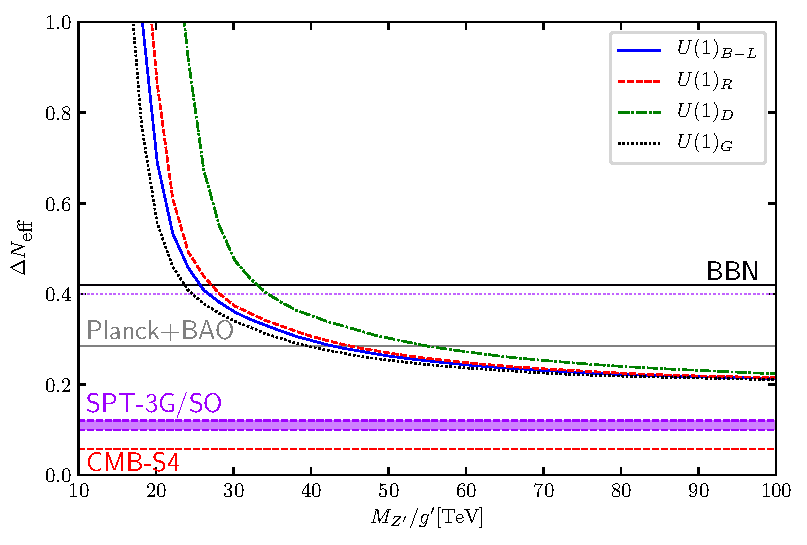
\includegraphics[scale=0.8]{D_Neff.pdf}
\caption{Contribution to the number of relativistic degrees of freedom ($\Delta N_{\text{eff}}$) in function of $M_{Z^{\prime}}/g^{\prime}$. The region above the gray line is excluded by the measurements in the Planck~\cite{Aghanim:2018eyx}. The horizontal dashed lines show the sensitivity of future experiments, SPT-3G/SO~\cite{Benson:2014qhw} and CMB-S4~\cite{Abitbol:2019nhf}. }
\label{fig:Neff}
\end{figure}

Prospect on $N_{\text{eff}}$~\cite{Abazajian:2019oqj}



\section{Collider constraints}
The recasting of the latest ATLAS results for the search of dilepton resonances using $139\ \text{fb}^{-1}$~\cite{Aad:2019fac} was done
in~\cite{Aad:2019fac} for the $\operatorname{U}(1)_{B-L}$ model.
The green region in Fig.~\ref{fig:u1blc} shows the excluded region at $95\%\ \text{C.L.}$. To ease the comparison with other results, we show the exclusion as function of $M_{Z'}/g_{BL}$. In particular, the limit from LEP for $\operatorname{U}(1)_{B-L}$ model is~\cite{Heeck:2014zfa}, 
\begin{align}
  M_{Z'}/g_{BL}>6.7\ \text{TeV}\,,&&\text{at $95\%$ C.L }
\end{align}

which is obtained from the search for effective four-lepton operators and valid for $M_{Z'}\gg 200\ \text{GeV}$. This constraint is relevant for $M_{Z'}>5.8\ \text{TeV}$, is shown in the excluded magenta region.

\begin{figure}
    \centering
    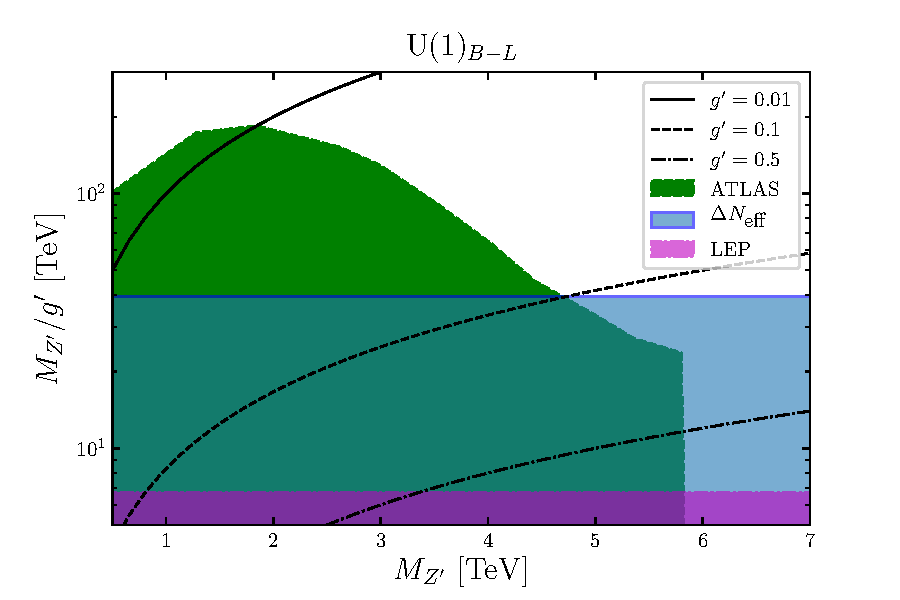
\includegraphics[scale=0.8]{u1blc}
    \caption{Constraints in the $\operatorname{U}(1)_{B-L}$ model.}
    \label{fig:u1blc}
\end{figure}

The constraint of $\Delta N_{\text{eff}}$ for $\operatorname{U}(1)_{B-L}$ is shown in the blue region and start to be better that current ATLAS limit for $M_{Z'}\gtrsim 4.8\ \text{TeV}$. Similar restrictions can be obtained for other values for the other models quoted in fig.~\ref{fig:Neff}.


\section{Discussion and summary}

\appendix



%\bibliographystyle{h-physrev4}
%\bibliographystyle{JHEP-2}
%\bibliographystyle{JHEP}
\bibliographystyle{apsrev4-1long}
%\bibliographystyle{apsrev4-1longdoi}
\bibliography{susy}



\end{document}

%%% Local Variables: 
%%% mode: latex
%%% TeX-master: "draft"
%%% ispell-local-dictionary: "american"
%%% End: 
